\documentclass{beamer}
\usetheme{Madrid} % Clean theme
\usepackage{listings}
\usepackage{xcolor}
\usepackage{graphicx}

\usepackage{gvv}

% Code listing style
\lstset{
  basicstyle=\ttfamily\footnotesize,
  keywordstyle=\color{blue},
  stringstyle=\color{orange},
  commentstyle=\color{green!60!black},
  breaklines=true,
  frame=single,
  showstringspaces=false
}

\title{MatGeo Assignment - Problem 1.5.12}
\author{EE25BTECH11024}
\institute{IIT Hyderabad}
\date{\today}

\begin{document}

% Title slide
\begin{frame}
  \titlepage
\end{frame}

% Problem statement
\begin{frame}{Problem Statement}
In what ratio does the point $P(-4, y)$ divide the line segment joining 
$A(-6,10)$ and $B(3,-8)$? Hence, find the value of $y$.
\end{frame}

% Solution using Rank Criterion (Slide 1)
\begin{frame}{Solution: Using the Rank Criterion}
\noindent
We are given three points:

\begin{align}
A = \myvec{-6 \\ 10}, \quad 
P = \myvec{-4 \\ y}, \quad 
B = \myvec{3 \\ -8}
\end{align}

\section*{Step 1: Using the rank condition for collinearity}

The points \(A, P, B\) are collinear if

\begin{align}
\text{rank}\big(\myvec{P-A & B-A}\big) = 1
\end{align}

Thus, the matrix is

\begin{align}
M = \myvec{2 & 9 \\ y-10 & -18}
\end{align}

Perform the row operations: $R_1 \leftarrow R_1/2$ and $R_2 \leftarrow R_2 - R_1(y-10)$  which results in

\end{frame}

% Solution using Rank Criterion (Slide 2)
\begin{frame}{Solution: }

\begin{align}
\myvec{1 & 9/2 \\ 0 & -9/2(y-6)}
\end{align}

If y is not equal to 6, then we perform $R_2 \leftarrow R_2/(-9/2(y-6))$ to get an identity matrix. But then the rank will be 2 \\
For the rank to be 1, the second row must be all zeros:

$
y - 6 = 0 \quad \Rightarrow \quad y = 6
$

---

\section*{Step 2: Finding \(k\)}

Using the vector formula,

\begin{align}
k = \frac{(\vec{A} - \vec{P})^\top(\vec{P} - \vec{B})}{\|\vec{P} - \vec{B}\|^2}
\end{align}

Substitute $y = 6$:
Compute the numerator:

\begin{align}
(\vec{A}-\vec{P})^\top (\vec{P}-\vec{B}) = (-2)(-7) + (4)(14) = 14 + 56 = 70
\end{align}

\end{frame}

% Solution using Rank Criterion (Slide 3)
\begin{frame}{Solution:}
Compute the denominator:

\begin{align}
\|\vec{P}-\vec{B}\|^2 = (-7)^2 + (14)^2 = 49 + 196 = 245
\end{align}

Thus,

\begin{align}
k = \frac{70}{245} = \frac{2}{7}
\end{align}

Therefore,
\begin{align}
\boxed{y = 6, \quad k = \frac{2}{7}}
\end{align}  
See the graphical representation in Figure 1.
\end{frame}


\begin{frame}{Resulting Graph}
\centering
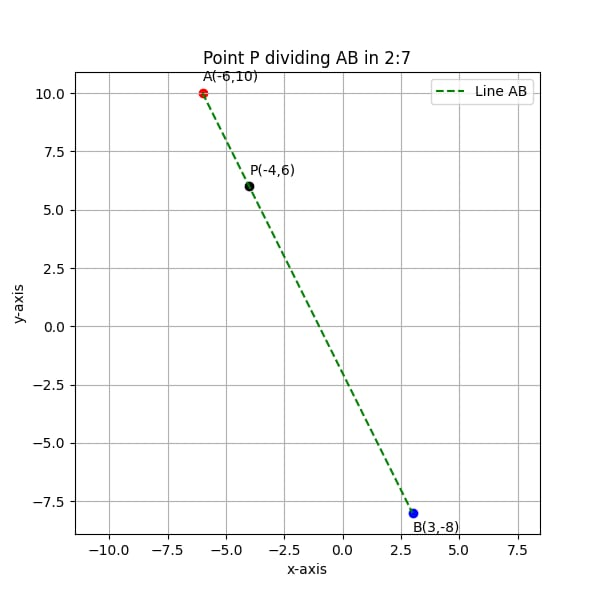
\includegraphics[width=0.6\linewidth]{figs/fig.jpg}
\end{frame}

% Python code 1
\begin{frame}[fragile]{Python Code: plot.py (Native)}
\begin{lstlisting}[language=Python]
import numpy as np
import matplotlib.pyplot as plt

# Given points
A = np.array([-6, 10])
B = np.array([3, -8])
P = np.array([-4, 6])   # Found from calculation

# Plotting
plt.figure(figsize=(6,6))
plt.plot([A[0], B[0]], [A[1], B[1]], 'g--', label="Line AB")
plt.scatter(*A, color="red")
plt.scatter(*B, color="blue")
plt.scatter(*P, color="black")

# Labels
plt.text(A[0], A[1]+0.5, "A(-6,10)", fontsize=10)
plt.text(B[0], B[1]-0.8, "B(3,-8)", fontsize=10)
plt.text(P[0], P[1]+0.5, "P(-4,6)", fontsize=10)
\end{lstlisting}
\end{frame}


\begin{frame}[fragile]{Python Code (Native Implementation – plot.py)}
\begin{lstlisting}[language=Python]
plt.xlabel("x-axis")
plt.ylabel("y-axis")
plt.title("Point P dividing AB in 2:7")
plt.legend()
plt.grid(True)
plt.axis("equal")
plt.savefig("fig.png")
plt.show()
\end{lstlisting}
\end{frame}

\begin{frame}[fragile]{C Code (Shared Library – find point.c)}
\begin{lstlisting}[language=C]
#include <stdio.h>

void find_point(double *px, double *py) {
    // A(-6,10), B(3,-8)
    double x1 = -6, y1 = 10, x2 = 3, y2 = -8;
    int m = 2, n = 7; // ratio

    *px = (m*x2 + n*x1) / (m+n);
    *py = (m*y2 + n*y1) / (m+n);
}
\end{lstlisting}
\end{frame}

% Python code 2
\begin{frame}[fragile]{Python Code: call.py (C + Python)}
\begin{lstlisting}[language=Python]
import ctypes
import numpy as np
import matplotlib.pyplot as plt

# Load shared object
so = ctypes.CDLL("./find_point.so")

# Prepare arguments
px = ctypes.c_double()
py = ctypes.c_double()

so.find_point(ctypes.byref(px), ctypes.byref(py))

A = np.array([-6, 10])
B = np.array([3, -8])
P = np.array([px.value, py.value])

# Plot
plt.figure(figsize=(6,6))
plt.plot([A[0], B[0]], [A[1], B[1]], 'g--', label="Line AB")
\end{lstlisting}
\end{frame}

\begin{frame}[fragile]{Python Code (C Integrated – call.py)
}
\begin{lstlisting}[language=Python]
plt.scatter(*A, color="red")
plt.scatter(*B, color="blue")
plt.scatter(*P, color="black")

plt.text(A[0], A[1]+0.5, "A(-6,10)", fontsize=10)
plt.text(B[0], B[1]-0.8, "B(3,-8)", fontsize=10)
plt.text(P[0], P[1]+0.5, f"P({px.value:.1f},{py.value:.1f})", fontsize=10)

plt.xlabel("x-axis")
plt.ylabel("y-axis")
plt.title("Point P from C code")
plt.legend()
plt.grid(True)
plt.axis("equal")
plt.show()
\end{lstlisting}
\end{frame}



\end{document}
